\section{MLPerf HPC}
{{\footnotesize
\begin{description}[labelwidth=5em, labelsep=1em, leftmargin=*, align=left, itemsep=0.3em, parsep=0em]
  \item[date:] 2021-10-20
  \item[version:] TODO
  \item[last\_updated:] 2021-10
  \item[expired:] unknown
  \item[valid:] yes
  \item[valid\_date:] TODO
  \item[url:] \href{https://github.com/mlcommons/hpc}{https://github.com/mlcommons/hpc}
  \item[doi:] TODO
  \item[domain:] Cosmology, Climate, Protein Structure, Catalysis
  \item[focus:] Scientific ML training and inference on HPC systems
  \item[keywords:]
    - HPC
    - training
    - inference
    - scientific ML
  \item[summary:] MLPerf HPC introduces scientific model benchmarks (e.g., CosmoFlow, DeepCAM) aimed at large-scale HPC evaluation with >10x performance scaling through system-level optimizations.

  \item[licensing:] TODO
  \item[task\_types:]
    - Training
    - Inference
  \item[ai\_capability\_measured:]
    - Scaling efficiency
    - training time
    - model accuracy on HPC
  \item[metrics:]
    - Training time
    - Accuracy
    - GPU utilization
  \item[models:]
    - CosmoFlow
    - DeepCAM
    - OpenCatalyst
  \item[ml\_motif:]
    - HPC/inference, HPC/training
  \item[type:] Framework
  \item[ml\_task:]
    - NA
  \item[solutions:] TODO
  \item[notes:] Shared framework with MLCommons Science; reference implementations included.

  \item[contact.name:] Steven Farrell (MLCommons)
  \item[contact.email:] unknown
  \item[results.links.name:] ChatGPT LLM
  \item[fair.reproducible:] Yes
  \item[fair.benchmark\_ready:] Yes
  \item[ratings.software.rating:] 0
  \item[ratings.software.reason:] Not analyzed. 

  \item[ratings.specification.rating:] 9.0
  \item[ratings.specification.reason:] Focused on structured/unstructured data pipelines; clearly defined tasks spanning analytics to AI; some scenarios lack hardware constraint modeling.

  \item[ratings.dataset.rating:] 9.0
  \item[ratings.dataset.reason:] Built from 13 real-world sources; structured for realistic big data scenarios; partially FAIR-compliant with documented data motifs.

  \item[ratings.metrics.rating:] 9.0
  \item[ratings.metrics.reason:] Covers data throughput, latency, and accuracy; quantitative and benchmark-ready.

  \item[ratings.reference\_solution.rating:] 8.0
  \item[ratings.reference\_solution.reason:] Many pipeline and model examples provided using Hadoop/Spark/Flink; setup effort varies by task and platform.

  \item[ratings.documentation.rating:] 8.0
  \item[ratings.documentation.reason:] Strong documentation with examples and task specifications; centralized support exists, but task-specific tuning may require domain expertise.

  \item[id:] mlperf\_hpc
  \item[Citations:] \cite{farrell2021mlperfhpcholisticbenchmark}
  \item[Ratings:]
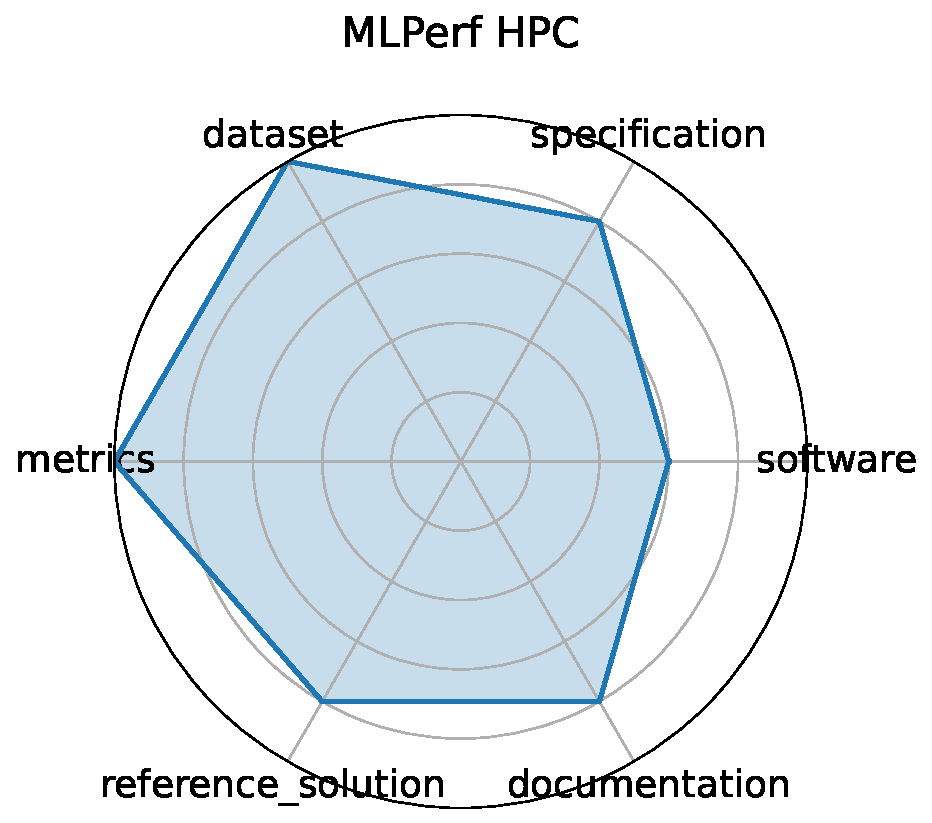
\includegraphics[width=0.2\textwidth]{mlperf_hpc_radar.pdf}
\end{description}
}}
\clearpage